% EN49 c01 | 原书 原书 p.1–11（PDF 12–22） | 第 1 章 §1.1–1.3
% 骨架文件：标题行已设定，正文由译者填写。每页起首用 % ===== 原书 p.N ===== 注释标记。
\section{引言}

\subsection{概述}

% ===== 原书 p.1 =====
泛言之，镜像对称是这样一个猜想中的关系：一个空间（A 侧）的辛几何，与它的“镜像”空间
（B 侧）的代数几何相对应。Kontsevich 在 [Kon95] 中猜想，这类联系源自同调镜像对称
（homological mirror symmetry，缩写 HMS）：复代数簇 $X$ 上的相干层范畴
$\operatorname{Coh}(X)$（它编码 $X$ 的闭子簇上的向量丛）与同维数镜像簇 $\check X$ 的
深谷范畴 $\cW(\check X)$（它编码 $\check X$ 的拉格朗日子流形及其相交）之间，应当存在
一种等价。人们还预期反方向也成立，即把镜像 $\check X$ 上的相干层范畴与原簇 $X$ 上的
深谷范畴联系起来。

\transnote{易错预警：原文 “putative equivalence” 中的 putative 意为“被假定的、尚待证明
的”，故译“应当存在一种等价”；HMS 至今没有一般证明，不宜译为“存在等价”。}

% ===== 原书 p.2 =====
起初，$X$ 与 $\check X$ 都被取为紧卡拉比–丘流形；如今 HMS 已被推广到远超其原始语境的
范围：一般型流形 [AAK16; Sei11; GKR17]、非凯勒流形 [War21]、非阿基米德解析空间，甚至
进入算术与同伦的领域。对我们而言特别重要的一种推广是到 Fano 簇 [HV00; AKO06; Sei02]：
它们的镜像是带全纯函数的簇，该函数称为 Landau--Ginzburg（LG）模型。带全纯映射到 $\C$
的凯勒流形，其深谷范畴称为 Fukaya--Seidel 范畴；这类范畴具有丰富的结构性质，而这些
性质编码在一个反常束（perverse schober）[KS14a] 的代数数据之中——反常束是反常层
（perverse sheaf）的范畴化版本。这些结构及其镜像，构成本论文的一条主线。

\transnote{背景直觉：卡拉比–丘情形两侧都是紧流形，是最初的设定；Fano 情形 B 侧的镜像
不再是簇本身，而是“簇加全纯函数”，即 LG 模型——这正是本文反复使用的对象。}
\transnote{含糊点拨：反常束（perverse schober）由 Kapranov--Schechtman 引入，是对
反常层取“范畴化”后的产物：把层的粘合数据换成范畴与函子的粘合数据。阅读时可先把它当作
“记账工具”，不必先掌握全部定义。}

HMS 的一处麻烦在于，有些簇可能根本没有镜像；即便存在镜像簇 $\check X$，镜像也可能不止
一个、维数互不相同，而且可能是奇异簇。在许多自然的镜像对称实例中（例如 $X$ 非紧时），
人们往往预期“内蕴”的镜像 $\check X$ 是奇异簇。人们理解光滑簇的镜像对称已取得惊人进
展；但在轨形情形之外，关于奇异簇 A 模型的镜像对称却少有论述，因为此时 $\check X$ 的深
谷范畴尚缺乏有原则的定义。对早期工作的进一步讨论见 §1.4。

此外，对任何由给定凯勒流形 $X$ 构造镜像空间的方法，一项主要诉求是：镜像的镜像应当回
到原来的凯勒流形；换言之，HMS 应当是一个对合。然而这立刻遇到困难：许多“内蕴”的镜像
构造自然给出奇异簇，而若不了解它们的深谷范畴，便难以继续推进。

\transnote{含糊点拨：“内蕴”的镜像（the ‘intrinsic’ mirror）指不依赖额外选择、由给定
数据自然给出的镜像构造；作者用引号提示这只是习惯说法，并非严格术语。}

% ===== 原书 p.3 =====
说明这些困难的一个重要例子——我们通篇都会用到——是 $(\C^*)^{n+1}$ 中的高维裤子
（pair of pants）
\[
\Pi_n=\{x_1+\cdots+x_{n+1}+1=0\}\subset(\C^*)^{n+1},
\]
其按内蕴方式构造的镜像，由 $\C^{n+1}$ 中的奇异超曲面 $\{z_1\cdots z_{n+1}=0\}$ 给出。
裤子是极仿射超曲面的基本构件；所谓极仿射超曲面，即 $(\C^*)^n$ 中的代数超曲面 $H$。
裤子在镜像对称中是基本的例子，因为借助热带几何的技巧，只要把这类超曲面分解为不同维数
的裤子之积，A 侧与 B 侧的计算往往就能化归为组合计数。因此，对那些依靠粘合技巧来证明
HMS 的途径而言，理解这类情形下的镜像对称至关重要。在本论文第二部分，我们考虑反方向的
镜像对称，此时裤子 $\Pi_n$ 位于 A 侧。不同维数的这些裤子的深谷范畴之间，由“提升”与
“限制”函子自然联系；我们证明在 HMS 之下，它们对应 Orlov 所构造的函子，后者联系不同
$n$ 的空间 $\{z_1\cdots z_{n+1}=0\}$ 上的相干层（见 §1.6）。

\transnote{易错预警：$\Pi_n$ 有 $n+1$ 个变量，故 $\Pi_n\subset(\C^*)^{n+1}$；其镜像是
$\C^{n+1}$ 中 $n+1$ 个坐标因子之积为零的奇异超曲面。指标 $n$ 与 $n+1$ 容易写错，回页图
核对时须逐字对照。}
\transnote{背景直觉：裤子是 $(\C^*)^{n+1}$ 中“一个仿射线性方程”定义的超曲面，也是构成
极仿射超曲面的最小单位；把超曲面作热带退化后，各块往往就是不同维数的裤子之积，故可由
组合数据（扇、多面体）算出两侧的量。}

在本论文第一部分，我们研究 Auroux 提出的奇异超曲面的深谷范畴的一种定义：把邻近光滑纤
维的深谷范畴，在 Seidel [Sei08b] 定义的某条自然变换处作范畴局部化，这条自然变换与绕奇
异纤维的单值性相关联。Auroux 的关键洞见是：超曲面本身的辛几何或许难以内蕴地理解；但只
要给定它的一个光滑化，邻近纤维便是完全良好的光滑辛流形，其深谷范畴还带有额外的代数数
据——一族由某些全纯截面计数给出的态射，它们记录了流形在趋向奇异纤维时有哪些部分发生
退化。

% ===== 原书 p.4 =====
按照反常束的哲学 [KS14b]，不变圈定理提示：在这些态射处作范畴局部化，便可得到奇异超曲
面的“深谷范畴”。正如 §1.3 将要说明的，这种在代数单值数据处作局部化的技巧，其几何适用
范围更广。Auroux 定义的精确版本将在 §2.3 给出。

\begin{figure}[htbp]
\centering
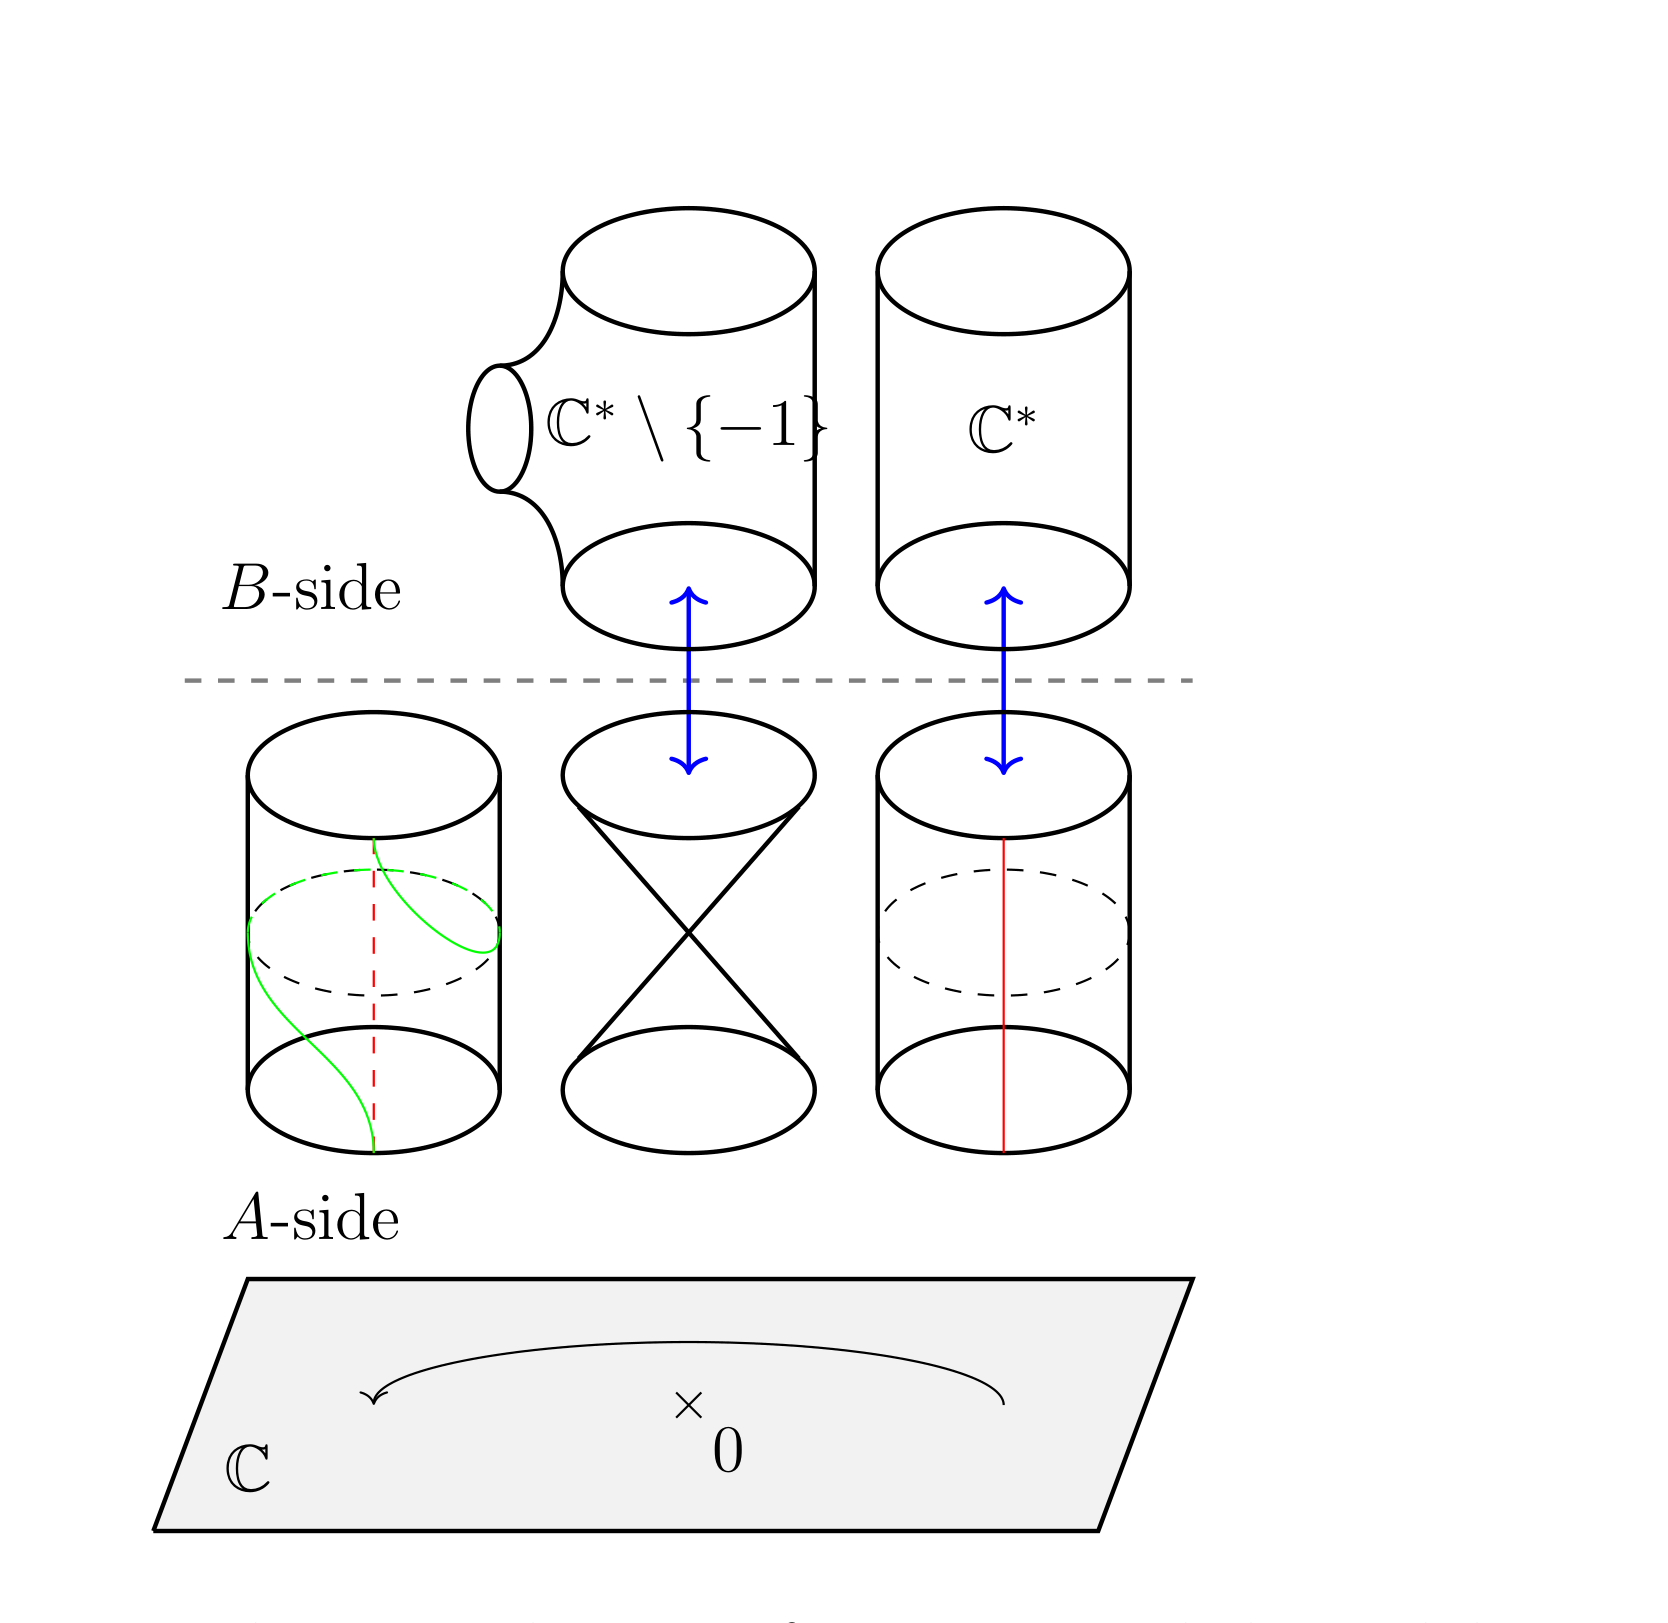
\includegraphics[width=0.60\textwidth]{figures/fig1_1.png}
\caption{裤子 $\Pi_1$ 与结点二次曲线 $\{xy=0\}$ 之间的镜像对称。}
\label{fig:pair-pants}
\end{figure}

最简单的例子是 $\Pi_1$，其镜像是 $\C^2$ 中的结点二次曲线 $\{xy=0\}$。该奇异超曲面的
光滑化是柱面 $\{xy=t\}$，绕 $t=0$ 的单值性由沿结点 vanishing cycle 的 Dehn twist 扭转
给出。HMS 中的一项标准计算给出：柱面的 wrapped Fukaya 范畴由 Laurent 多项式环
$\C[z^{\pm1}]$ 上的有限生成模给出，而 Dehn twist 扭转诱导的自然变换对应乘 $1+z$。

% ===== 原书 p.5 =====
在这条自然变换处作局部化，等于让 $1+z$ 可逆；这确实给出裤子 $\C^*\setminus\{-1\}$ 上的
函数环（见图 \ref{fig:pair-pants}）。

\transnote{背景直觉：柱面 $\{xy=t\}$ 的 wrapped Fukaya 范畴等价于 $\C[z^{\pm1}]$ 上的
有限生成模范畴，生成元 $z$ 对应绕柱面一周的拉格朗日圆圈；乘 $1+z$ 这条自然变换把
$\C[z^{\pm1}]$ 换成 $\C[z^{\pm1},(1+z)^{-1}]$，后者正是 $\C^*\setminus\{-1\}$ 上的函数
环。作者借此把“局部化”落到一个可手算的例子。}

按通常表述，HMS 还有一处问题：它在某种意义上提法不够确定——给定一对范畴之间可能存在许
多等价，其中一些显然涉及作选择。例如，许多 HMS 证明的做法是：在 A 侧与 B 侧各选
一组生成元，再匹配它们的自同态代数。我们如何锁定某一个特定的 HMS 等价？一种回答是：应
当要求 HMS 把 A 侧与 B 侧自然定义的函子相互交织。这类结果此前已见于文献，例如
[HH22; Han19; Nad19b; Can20; HK21]，以及 Cannizzo--Azam--Lee--Liu 的在研工作；此外，
人们早已知道（始于 [PZ98; Fuk02]）阿贝尔簇的镜像对称尊重幺半结构。在本论文第二部分，
我们研究通常镜像对称定理的一种强化：函子性镜像对称试图证明，我们不仅有一个镜像等价，
而且有正确的镜像等价，即它把 A 侧与 B 侧自然定义的函子相互交织。

\transnote{含糊点拨：“正确的镜像等价”不是指唯一性，而是指所取的等价同时与两侧的自然
函子相容；作者把这一要求称为函子性镜像对称，并以“交织”（intertwine）说明函子与等价
之间的交换关系。}

Auroux 在 [Aur18] 中注意到：极仿射超曲面 $H$ 的补集 $(\C^*)^n\setminus H$ 本身是
$(\C^*)^{n+1}$ 中的极仿射超曲面，并且 $H$ 的镜像对称应当与 $(\C^*)^n\setminus H$ 的镜
像对称相关联。在本论文第二部分（与 Benjamin Gammage 的合作工作），我们发现极仿射超曲
面的补集其实有两个自然镜像，其中之一是导出概型。这两个镜像由一个以 Orlov 导出
Kn{\"o}rrer 周期性为中介的非几何等价相联系。

% ===== 原书 p.6 =====
在本论文第二部分，我们随后用这些想法证明 Auroux 的函子性镜像对称猜想：极仿射超曲面及
其补集的同调镜像对称，尊重 A 侧与 B 侧某些自然定义的函子。

\subsection{奇异超曲面}

在本论文第一部分，我们证明：采用 Auroux 的定义，奇异超曲面（在\emph{大复结构极限}处）
的深谷范畴确实满足所预期的同调镜像对称等价。我们还证明 Orlov 的一个猜想：这些奇异超曲
面的深谷范畴满足其\emph{导出} Kn{\"o}rrer 周期性定理的辛类比。这些结果为研究 HMS 开辟
了新途径——使我们能够研究非常一般的一类奇异簇的 A 模型。此外，它还解释了某些簇何以会
有若干个不同维数的镜像。

概括 Auroux 的定义如下。设 $X$ 是 Stein 流形。对只有一个奇异纤维（位于 $0$ 上方）的奇
异辛纤维丛 $f\colon X\to\C$，Seidel [Sei09b; Sei12] 定义了一条自然变换
$s\colon\mu\to\id$，其中 $\mu$ 是作用在一般纤维的 wrapped Fukaya 范畴
$\cW(f^{-1}(t))$ 上的顺时针单值函子（定义见 §2）。Auroux 提出了下述奇异纤维的 wrapped
Fukaya 范畴的定义：

\begin{definition}[Auroux]\label{def:sing-fuk}
设奇异辛纤维丛 $f\colon X\to\C$ 恰有一个奇异纤维，位于 $0$ 上方。则 $f^{-1}(0)$ 的
wrapped Fukaya 范畴定义为：在自然变换 $s\colon\mu\to\id$ 处，对充分小的 $t\neq0$ 取邻
近纤维 $f^{-1}(t)$ 的 wrapped Fukaya 范畴的局部化：
\[
D\cW(f^{-1}(0))=D\cW(f^{-1}(t))[s^{-1}].
\]
\end{definition}

% ===== 原书 p.7 =====
此处是 [LO06] 意义下 $A_\infty$ 范畴的局部化，而 $D$ 表示扭复形的范畴。这一定义也可推
广到单调纤维的情形，或任何 Seidel 自然变换有定义的场合。

\transnote{易错预警：$D$ 是扭复形范畴的记号，与后文的 $D^\pi$（幂等完备的扭复形范畴）
不同；两者在原文中都是数学斜体的 $D$，不要误排成花体 $\cD$（花体 $\cD$ 在本论文中另指
一个满子范畴，见 §1.3.1 末段）。}

在本论文第一部分，我们将证明若干结果，以说明这确实就是奇异超曲面的深谷范畴的正确定义：
Orlov 导出 Kn{\"o}rrer 周期性定理的一个 A 侧类比（定理 \ref{thm:knorrer}），以及若干
大复结构极限处的同调镜像对称等价（定理 \ref{thm:lcsl}）。这些结果将在随后各节详述。

我们将在 §2.3 给出一个启发式说明，解释定义 \ref{def:sing-fuk} 与 Biran--Cornea 拉格朗
日配边群的一个版本之间何以有非常自然的关系。此外还可以构造“邻近圈”函子的一个自然类
比，它把拉格朗日子流形从奇异纤维的去心邻域的 wrapped Fukaya 范畴，限制到奇异纤维自身
的 wrapped Fukaya 范畴（见 §8）。

\subsection{Kn{\"o}rrer 周期性}

关于奇异超曲面深谷范畴的第一个定理，其灵感来自 Orlov 的导出 Kn{\"o}rrer 周期性定理
[Orl06a, Corollary 3.2]。该定理断言：若 $X$ 是光滑拟射影簇，$f\colon X\to\C$ 是正则函
数且 $f^{-1}(0)$ 光滑，则存在范畴等价
\[
\operatorname{Coh}(f^{-1}(0))\to\operatorname{Sing}(X\times\C,zf),
\]
其中 $z$ 是 $\C$ 上的坐标。

% ===== 原书 p.8 =====
[Orl06a] 虽在 $f^{-1}(0)$ 光滑的情形下陈述该定理，但结论对任意超曲面都成立（见 §6.1）：
因此它使我们能用光滑簇 $X\times\C$ 上的 LG 模型来研究这类奇异超曲面。Orlov 在 [Orl06a]
中猜想：同一关系对 A 模型也应成立；与 Orlov 的结果类比，我们或可期望 $f^{-1}(0)$ 的
wrapped Fukaya 范畴，等价于 Landau--Ginzburg 模型 $(X\times\C,zf)$ 的（逐纤维缠绕的）
Fukaya--Seidel 范畴，记作 $\cW(X\times\C,zf)$。这是我们的第一个主要结果。

\transnote{含糊点拨：$\operatorname{Sing}$ 记号的严格含义见 §6.1；在那里作者用矩阵分解
范畴给出它的具体模型。此处只需知道它是 B 侧一个只依赖 LG 模型 $(X\times\C,zf)$ 的范畴，
从而使“奇异纤维的 A 侧”有了“光滑簇上的 LG 模型”这一替身。}

\begin{theorem}[{导出 Kn{\"o}rrer 周期性}]\label{thm:knorrer}
设 $X$ 是光滑仿射簇，带嵌入 $X\to\C^N$，该嵌入在 $X$ 上诱导 Stein 结构；设
$f\colon X\to\C$ 是 $\C^N$ 上多项式函数的限制。若 $f$ 只有一个临界纤维 $f^{-1}(0)$，
则对充分小的 $t\neq0$，存在 $A_\infty$ 范畴的拟等价
\[
D^\pi\cW(f^{-1}(t))[s^{-1}]\to D^\pi\cW(X\times\C,zf).
\]
\end{theorem}

此处 $D^\pi$ 表示扭复形的幂等完备化；我们预期，若不取幂等完备化，该结果不成立。几何假
设几乎肯定可以减弱，但现有的假设已足以用于镜像对称的应用。

% ===== 原书 p.9 =====
注意，对 LG 模型而言，这是与奇点理论中通常考虑的“悬置”或“周期性”不同的一种形式（比
较 [Sei09a]）。

\transnote{含糊点拨：原文强调“不同的一种形式”，指通常的悬置把一个 LG 模型换成另一个、
不改变奇异纤维的等价类；而这里把奇异纤维 $f^{-1}(0)$ 的范畴与高一维的 LG 模型
$(X\times\C,zf)$ 的范畴等同起来，方向相反，故作者特别提醒不要混同。}

上述结果未必局限于奇异超曲面。对奇异完全交，我们可以作如下定义：

\begin{definition}\label{def:sing-ci}
设 $f_1,\dots,f_k\colon X\to\C$ 是 Stein 流形上的全纯函数，且当
$t_1,\dots,t_k\neq0$ 时，交 $f_1^{-1}(t_1)\cap\cdots\cap f_k^{-1}(t_k)$ 光滑。则定义
\[
D\cW(f_1^{-1}(0)\cap\cdots\cap f_k^{-1}(0))
=D\cW(f_1^{-1}(t_1)\cap\cdots\cap f_k^{-1}(t_k))[s_1^{-1},\dots,s_k^{-1}],
\]
其中 $s_i$ 是 $f_i$ 绕 $t_i=0$ 的单值性给出的自然变换，$t_i$ 充分小。
\end{definition}

把我们的证明迭代下去，我们还预期主定理可以简单推广到奇异完全交：

\begin{conjecture}\label{conj:sing-ci}
在关于 $f_1,\dots,f_k$ 的适当假设下，存在 $A_\infty$ 范畴的拟等价
\[
D^\pi\cW(f_1^{-1}(0)\cap\cdots\cap f_k^{-1}(0))
\simeq D^\pi\cW(X\times\C^k,z_1f_1+\cdots+z_kf_k),
\]
其中 $z_1,\dots,z_k$ 是 $\C^k$ 上的坐标。
\end{conjecture}

下文将讨论如何通过推广本论文的结果来证明这一猜想。

\transnote{易错预警：定义 \ref{def:sing-ci} 的显示公式中，左侧各 $f_i$ 取 $0$，右侧各
$f_i$ 取 $t_i$，且局部化要同时在 $k$ 条自然变换处进行，写 $[s_1^{-1},\dots,s_k^{-1}]$；
不要漏掉下标或误写成单个 $s^{-1}$。}

\subsubsection{Kn{\"o}rrer 周期性定理的证明概要}

% ===== 原书 p.10 =====
我们首先在我们的框架下，给出 Abouzaid--Auroux--Katzarkov 一个定理
[AAK16, Corollary 7.8] 的强化形式之证明，该结果或许有独立的价值：

\begin{theorem}[{Abouzaid--Auroux--Katzarkov 等价}]\label{thm:aak-equiv}
设 $X$ 是光滑仿射簇，带嵌入 $X\to\C^N$，该嵌入在 $X$ 上诱导 Stein 结构；设
$f\colon X\to\C$ 是 $\C^N$ 上多项式函数的限制。若 $f$ 只有一个临界纤维 $f^{-1}(0)$，
则对充分小的 $t\neq0$，存在 $A_\infty$ 范畴的拟等价
\[
T\colon\cW(f^{-1}(t))\to\cW(X\times\C,z(f-t)),
\]
它由在奇异轨迹 $f^{-1}(t)$ 中的可容拉格朗日子流形上取顶针给出。
\end{theorem}

\transnote{背景直觉：顶针（thimble）是沿一条路径“扫过”的拉格朗日圆盘，其边界落在
Lefschetz 纤维的消失圈上；作者用“在可容拉格朗日子流形上取顶针”描述这个函子 $T$，直观
上就是把 B 侧的 LG 模型沿临界轨迹切出的拉格朗日球面搬到 A 侧。}

在 [AAK16] 中，人们预期这是一个范畴等价，其前提是 Abouzaid--Ganatra [AG] 的一个生成性
结果，而后者应当由命题 \ref{prop:3-0-5} 推出。类似的结果可参看 [AS15, Lemma A.26]。这
一定理或可视为 LG--CY 对应的开弦类比。

\transnote{含糊点拨：LG--CY 对应把 LG 模型的 B 侧与一个卡拉比–丘流形的 A 侧联系起来；
这里是它的“开弦”版本，即把两侧的范畴（而非仅数值不变量）进行比较。}

还有这一陈述的相对版本，它针对逐纤维带停点的 Fukaya--Seidel 范畴，并镜像 Orlov 的一个
结果：

\begin{theorem}\label{thm:relative}
设 $X$ 是光滑仿射簇，带嵌入 $X\to\C^N$，该嵌入在 $X$ 上诱导 Stein 结构；设
$f,g\colon X\to\C$ 都是 $\C^N$ 上多项式函数的限制。若 $f$ 只有一个临界纤维
$f^{-1}(0)$，则对充分小的 $t\neq0$，存在全忠实函子
\[
\cW(f^{-1}(t),g)\to\cW(X\times\C,z(f-t),g).
\]
\end{theorem}

% ===== 原书 p.11 =====
此处第二个范畴关于 $g$ 逐纤维带停点，详见定义 \ref{def:4-1-1}。

由此还应能推出定理 \ref{thm:knorrer} 的相对版本，进而推出猜想 \ref{conj:sing-ci}：

\begin{conjecture}\label{conj:relative}
设 $f\colon X\to\C$ 是 Stein 流形 $X$ 上的全纯函数，且恰有一个临界纤维 $f^{-1}(0)$；
设 $g\colon X\to\C$ 是另一全纯函数。则对充分小的 $\delta,|t|>0$，存在 $A_\infty$ 范畴
的拟等价
\[
D^\pi\cW(f^{-1}(t),g)[s^{-1}]\to D^\pi\cW(X\times\C,zf+\delta g).
\]
\end{conjecture}

我们随后将在 §3 说明：通过仔细分析一般纤维在 $t$ 变化时的 Liouville 几何，从
$(X\times\C,z(f-t))$ 过渡到 $(X\times\C,zf)$ 可以改述为一次去停点（stop removal）。于是，
由 [GPS19; Syl19a] 的去停点定理，范畴 $\cW(X\times\C,zf)$ 可由范畴
$\cW(X\times\C,z(f-t))$ 对一个由环绕圆盘组成的满子范畴 $\cD$ 取商得到。最后，我们在 §4
证明：在定理 \ref{thm:aak-equiv} 的函子 $T$ 之下，$\cW(f^{-1}(t))$ 上自然变换
$\mu\to\id$ 的各锥的本质像，用 K{\"u}nneth 型论证可分裂生成与 $\cD$ 相同的满子范畴。
于是得到定理 \ref{thm:knorrer}。

\transnote{含糊点拨：停点（stop）是流形上允许拉格朗日对象“终结”的边界区域；把停点去掉
（stop removal）会使范畴变小，在形式上表现为对某个满子范畴取商。作者在此把
$z(f-t)$ 到 $zf$ 的变化解释为停点的移动，正是不变量在此处的几何来源。}

